%!TEX root = ../thesis.tex

\chapter{Analyse}

Dieses Kapitel beschäftigt sich mit der Analyse, was genau Tracing ist und welche Anwendungen es bereits in diesem Gebiet gibt. Außerdem werden Anforderungen dargelegt und durch Szenarien weiter erläutert.

\section{Tracing} 

Tracing beschreibt eine spezielle Form des Loggings, bei der Daten gesammelt werden, um den Ablauf eines Programms rekonstruieren zu können. Dies ermöglicht im Fehlerfall den Entwicklern nachvollziehen zu können, wo und wieso welches Problem aufgetreten ist. Die erzeugten Daten beim tracing werden als Programmtrace - oder kurz Trace - bezeichnet, was sich ins Deutsche als "`Spur"' übersetzen lässt. Tracing stellt die umfassendste Art des Loggings dar, da bis ins kleinste Detail die Ausführung protokolliert wird. Aus diesem Grund ist sie im produktiven Betrieb auch ungeeignet, da Massen an Daten erzeugt werden.

Ein Vorteil im Vergleich zum herkömmlichen Debugging, bei dem die Ausführung angehalten wird, ist dass der Einfluss auf die Thread-Synchronisierung minimal gehalten wird. Die Ausgaben haben nur einen geringen Einfluss auf einzelne Ausführungszeiten. Der Nachteil ist wiederum, dass Programme meist erst analysiert werden, wenn deren Ausführung bereits beendet ist. Somit sind Reaktionen auf die spezifischen Zustände schwerer realisierbar.

Diese Technik ist auch einsetzbar, um Programmieranfängern den Ablauf ihrer Programme zu vermitteln, besonders wenn der textuelle Trace von grafischen Anwendungen visualisiert wird. Diese können damit ohne viel Aufwand oder Kenntnis der Werkzeuge selbständig Programmfehler nachvollziehen und nach Lösungen suchen.

\section{Ähnliche Anwendungen} 

Zu Anwendungen, die solche Visualisierung bereits umgesetzt haben, zählen "`Jeliot 3"' für Java und "`Python Tutor"' für Python, Java, C und C++.

Jeliot ist eine Software, mit der lokale Programme analysiert werden können. Jedoch hat das Projekt seit 2007 keine Updates erhalten und ist deshalb mit Java 1.4 entwickelt worden. Moderne Programmierkonstrukte, die erst mit späteren Versionen eingeführt wurden, werden deshalb nicht unterstützt. Da das Programm zuerst ohne Interaktionsmöglichkeit ausgeführt wird, sind keine Eingaben möglich. Der gesamte Code muss in einem File sein um ausgeführt zu werden. Sind alle diese Randbedingungen erfüllt, kann damit die Ausführung schrittweise untersucht werden. Dabei werden Konstanten, der aktuelle Stack-Trace sowie Details aller Variablen und Methoden-Aufrufe visualisiert. Jeliot legt hier besonders Wert auf die Darstellung von Vererbungsstrukturen.

\begin{figure}[h]
	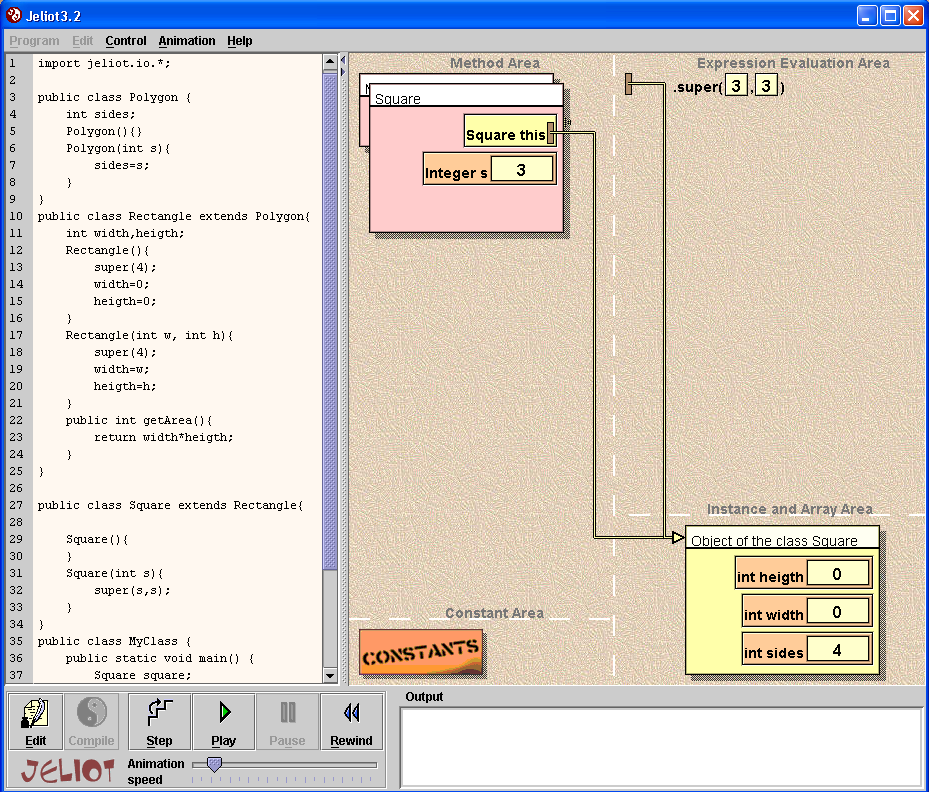
\includegraphics[width=\textwidth]{analyse/bilder/jeliot3.png}
	\caption{Oberfläche von Jeliot 3 (Quelle: http://cs.joensuu.fi/jeliot/images/jeliot3.2.png)}
\end{figure}

Python Tutor ist ein Online-Tool, welches Programme in verschiedenen Sprachen visualisieren kann. Bei Java gibt es dabei ähnliche Einschränkungen wie bei Jeliot:
\begin{itemize}
	\item Die Ausführung kann nur mit Java Version 1.8 erfolgen
	\item Es ist nicht möglich, Parameter an das Programm zu übergeben oder interaktive Eingaben zu machen
	\item Der Code muss in einem einzelnen Textfeld eingegeben werden
	\item Die maximale Ausführungszeit ist auf 10 Sekunden limitiert
	\item Es können nur die auf dem Server verfügbaren Bibliotheken verwendet werden
\end{itemize}

Auch hier erfolgt die Anzeige in einem übersichtlichen Format, mit Visualisierung von Zeigern und den Methoden auf dem Stack. Wichtig zu beachten ist jedoch, dass die Ausführung sehr langsam erfolgt. Selbst einfache Programme benötigen meist über eine Sekunde zur Ausführung.

\begin{figure}[h]
	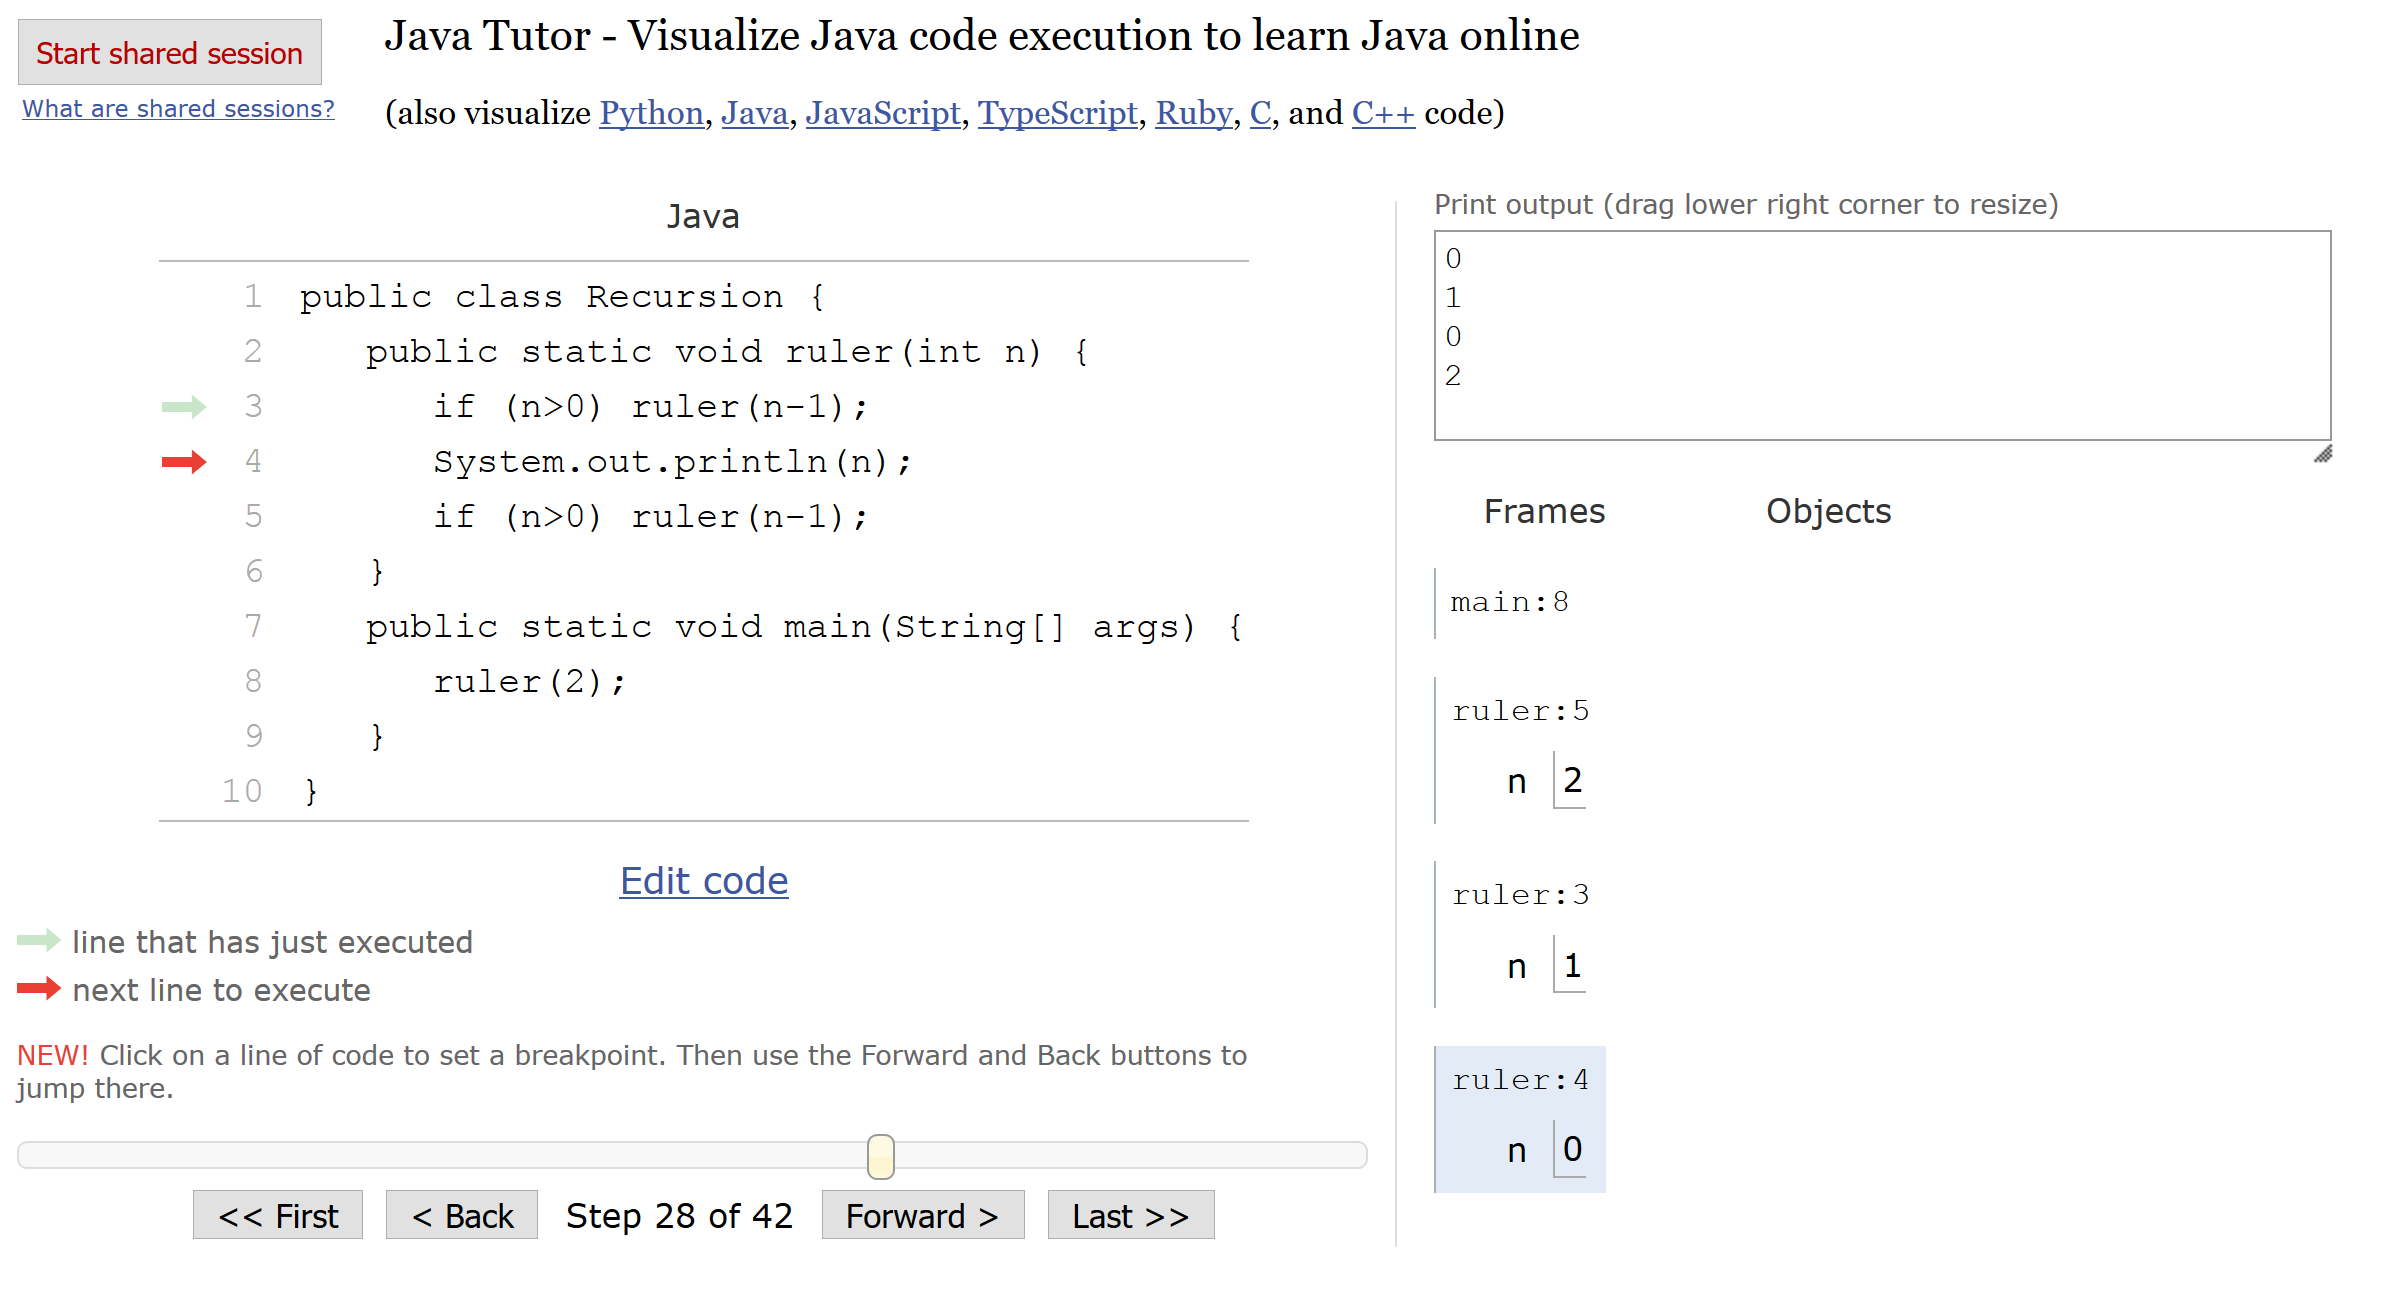
\includegraphics[width=\textwidth]{analyse/bilder/pythonTutor.png}
	\caption{Oberfläche von Python Tutor (Quelle: eigener Screenshot)}
\end{figure}

\section{Anforderungen} 
\label{sec:anforderungen}

Ziel dieser Arbeit ist jedoch nicht eine visuelle Darstellung, sondern lediglich die Möglichkeit einer textuellen Ausgabe für simple Programme, wie sie ein Programmieranfänger entwickelt. Die wichtigsten Anforderungen sind wie folgt definiert:

\begin{itemize}
	\item Erstellungen eines textuellen, menschlich lesbaren Programmtrace
	\item Keine Änderungen am Quelltext notwendig
	\item Kommandozeilen basiertes Interface
	\item Intuitive Benutzbarkeit
	\item Auswahlmöglichkeit von verschiedenen Optionen zur Erstellung des Trace
	\item Leichtgewichtig - keine Installation notwendig
	\item Erweiterbares Design, in das weitere Funktionen integriert werden können
\end{itemize}

Alle diese Anforderungen zielen auf ein simples Werkzeug für Anfänger ab, welches einfach zu benutzen ist, gleichzeitig aber Potenzial für komplexere Erweiterungen bietet.

\section{Szenario} 

Für einen möglichen Anwendungsfall nehmen wir das Programm in Listing~\ref{code:falscheSchleife} an. Wie einfach zu erkennen ist, wurde bei der Bedingung ein falscher Vergleichsoperator verwendet, weshalb "`7"' anstelle von "`10"' ausgegeben wird.

\lstinputlisting[language=Java,label=code:falscheSchleife,caption=Anfänger Programm mit Problem in Schleife]{analyse/wrongLoop.java}

Hier sollte ein einfacher Aufruf an Klara genügen, um angezeigt bekommen zu können, dass nur die Zeilen 3, 4 und 6 ausgeführt werden. Dies sollte als Information genügen, um das Problem zu lokalisieren.

Ein anderes Beispiel ist in Listing~\ref{code:falscheIf} zu sehen. Hier wird eine Variable zugewiesen und dann geprüft. Jedoch erfolgt dies nicht identisch, als würde die gesamte Rechnung in einem Schritt ausgeführt, weshalb das Ergebnis 50 und nicht 22 ist.

\lstinputlisting[language=Java,label=code:falscheIf,caption=Anfänger Programm mit Problem bei Variable]{analyse/wrongIf.java}

Hier sollte von Klara ausgegeben werden, das der Variable \code{r} zuerst "`5"' und dann "`50"' zugewiesen wird. Somit sollte für einen Entwickler nachvollziehbar sein, dass direkt eine Multiplikation mit 10 stattfindet und somit ein unterschied zu \code{r = r * 3 + 7} besteht.